\documentclass[tikz,border=8mm]{standalone}
\usetikzlibrary{shadows.blur}

\begin{document}
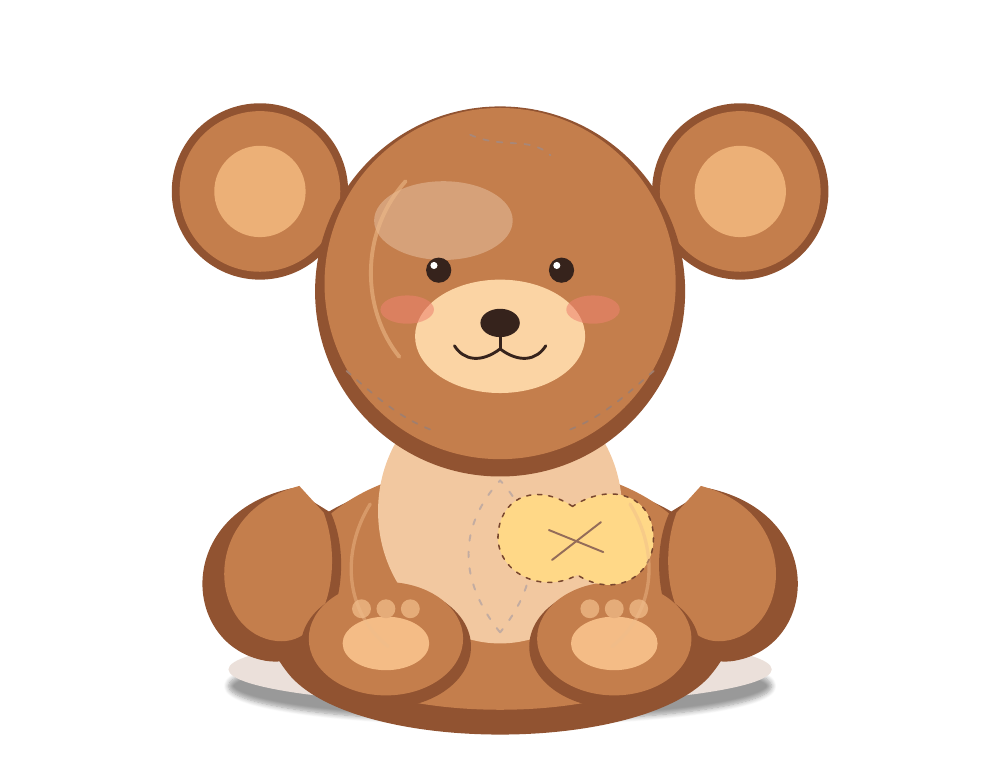
\begin{tikzpicture}[x=1cm,y=1cm,line cap=round,line join=round]

\definecolor{fur}{RGB}{196,126,76}
\definecolor{furDark}{RGB}{145,83,49}
\definecolor{furLight}{RGB}{236,176,119}
\definecolor{muzzle}{RGB}{251,212,164}
\definecolor{paw}{RGB}{244,188,134}
\definecolor{patch}{RGB}{255,216,135}
\definecolor{stitch}{RGB}{121,71,47}
\definecolor{eye}{RGB}{54,35,28}
\definecolor{blush}{RGB}{238,130,111}

\path[use as bounding box] (-6,-4.2) rectangle (6,4.8);

\fill[furDark!18, blur shadow={shadow blur steps=8, shadow xshift=0pt, shadow yshift=-6pt}]
  (0,-3.35) ellipse (3.45 and .45);

% ears
\fill[furDark] (-3.05,2.72) circle (1.12);
\fill[furDark] (3.05,2.72) circle (1.12);
\fill[fur] (-3.05,2.72) circle (1.02);
\fill[fur] (3.05,2.72) circle (1.02);
\fill[furLight] (-3.05,2.72) circle (.58);
\fill[furLight] (3.05,2.72) circle (.58);

% body
\fill[furDark]
  (0,-.85) .. controls (-2.75,-.88) and (-3.55,-2.42) .. (-2.65,-3.45)
  .. controls (-1.75,-4.42) and (1.75,-4.42) .. (2.65,-3.45)
  .. controls (3.55,-2.42) and (2.75,-.88) .. (0,-.85) -- cycle;
\fill[fur]
  (0,-.72) .. controls (-2.52,-.78) and (-3.16,-2.34) .. (-2.35,-3.24)
  .. controls (-1.55,-4.07) and (1.55,-4.07) .. (2.35,-3.24)
  .. controls (3.16,-2.34) and (2.52,-.78) .. (0,-.72) -- cycle;

% belly softness
\fill[furLight!70]
  (0,-1.34) ellipse (1.55 and 1.68);
\draw[stitch!45, line width=.7pt, dash pattern=on 2pt off 4pt]
  (0,-2.88) .. controls (-.55,-2.2) and (-.52,-1.52) .. (0,-.95)
  .. controls (.52,-1.52) and (.55,-2.2) .. (0,-2.88);

% arms
\fill[furDark] (-2.65,-1.05) .. controls (-4.15,-1.38) and (-4.05,-3.05) .. (-2.98,-3.24)
  .. controls (-2.12,-3.38) and (-1.82,-2.08) .. (-2.15,-1.36) -- cycle;
\fill[furDark] (2.65,-1.05) .. controls (4.15,-1.38) and (4.05,-3.05) .. (2.98,-3.24)
  .. controls (2.12,-3.38) and (1.82,-2.08) .. (2.15,-1.36) -- cycle;
\fill[fur] (-2.55,-1.02) .. controls (-3.82,-1.35) and (-3.7,-2.82) .. (-2.9,-2.98)
  .. controls (-2.2,-3.12) and (-1.98,-2.05) .. (-2.24,-1.36) -- cycle;
\fill[fur] (2.55,-1.02) .. controls (3.82,-1.35) and (3.7,-2.82) .. (2.9,-2.98)
  .. controls (2.2,-3.12) and (1.98,-2.05) .. (2.24,-1.36) -- cycle;

% legs
\fill[furDark] (-1.45,-3.06) ellipse (1.08 and .78);
\fill[furDark] (1.45,-3.06) ellipse (1.08 and .78);
\fill[fur] (-1.45,-2.96) ellipse (.98 and .72);
\fill[fur] (1.45,-2.96) ellipse (.98 and .72);
\fill[paw] (-1.45,-3.02) ellipse (.55 and .34);
\fill[paw] (1.45,-3.02) ellipse (.55 and .34);
\foreach \x in {-1.76,-1.45,-1.14} \fill[paw!85!furDark] (\x,-2.58) circle (.12);
\foreach \x in {1.14,1.45,1.76} \fill[paw!85!furDark] (\x,-2.58) circle (.12);

% head
\fill[furDark] (0,1.45) circle (2.35);
\fill[fur] (0,1.55) circle (2.23);
\fill[furLight!35, opacity=.35] (-.72,2.35) ellipse (.88 and .5);

% face
\fill[muzzle] (0,.88) ellipse (1.08 and .72);
\fill[eye] (-.78,1.72) circle (.16);
\fill[eye] (.78,1.72) circle (.16);
\fill[white] (-.84,1.78) circle (.045);
\fill[white] (.72,1.78) circle (.045);
\fill[blush, opacity=.55] (-1.18,1.22) ellipse (.34 and .18);
\fill[blush, opacity=.55] (1.18,1.22) ellipse (.34 and .18);

\fill[eye] (0,1.05) ellipse (.25 and .18);
\draw[eye, line width=1.15pt] (0,.88) -- (0,.72);
\draw[eye, line width=1.05pt] (0,.72) .. controls (-.24,.54) and (-.46,.57) .. (-.58,.76);
\draw[eye, line width=1.05pt] (0,.72) .. controls (.24,.54) and (.46,.57) .. (.58,.76);

% patch
\fill[patch] (.92,-1.28)
  .. controls (.47,-.98) and (.04,-1.15) .. (-.02,-1.58)
  .. controls (-.1,-2.08) and (.5,-2.42) .. (.98,-2.15)
  .. controls (1.5,-2.48) and (2.02,-2.12) .. (1.94,-1.58)
  .. controls (1.88,-1.12) and (1.37,-.98) .. (.92,-1.28) -- cycle;
\draw[stitch, line width=.55pt, dash pattern=on 1.5pt off 2.5pt]
  (.92,-1.28)
  .. controls (.47,-.98) and (.04,-1.15) .. (-.02,-1.58)
  .. controls (-.1,-2.08) and (.5,-2.42) .. (.98,-2.15)
  .. controls (1.5,-2.48) and (2.02,-2.12) .. (1.94,-1.58)
  .. controls (1.88,-1.12) and (1.37,-.98) .. (.92,-1.28) -- cycle;
\draw[stitch!80, line width=.7pt] (.62,-1.58) -- (1.31,-1.86);
\draw[stitch!80, line width=.7pt] (1.28,-1.48) -- (.66,-1.96);

% seams and stitches
\draw[stitch!70, line width=.65pt, dash pattern=on 2pt off 3pt]
  (-1.95,.44) .. controls (-1.56,.1) and (-1.28,-.16) .. (-.82,-.33);
\draw[stitch!70, line width=.65pt, dash pattern=on 2pt off 3pt]
  (1.95,.44) .. controls (1.56,.1) and (1.28,-.16) .. (.82,-.33);
\draw[stitch!65, line width=.65pt, dash pattern=on 2pt off 3pt]
  (-.38,3.44) .. controls (.05,3.25) and (.36,3.43) .. (.64,3.18);

% soft highlights
\draw[furLight!85, line width=1.4pt, opacity=.55]
  (-1.2,2.85) .. controls (-1.8,2.18) and (-1.75,1.2) .. (-1.28,.62);
\draw[furLight!85, line width=1.2pt, opacity=.45]
  (-1.65,-1.25) .. controls (-2.02,-1.85) and (-1.98,-2.62) .. (-1.42,-3.06);
\draw[furLight!85, line width=1.2pt, opacity=.45]
  (1.65,-1.25) .. controls (2.02,-1.85) and (1.98,-2.62) .. (1.42,-3.06);

\end{tikzpicture}
\end{document}
